\documentclass[polish,envcountsect,10pt]{beamer}
\usetheme{metropolis}
\usepackage[T1]{fontenc}
\usepackage{polski}
\usepackage{babel}
\usepackage{tikz}
\usepackage{graphicx}
\usepackage{xcolor}
\usepackage{algorithm}
\usepackage{algpseudocode}
\graphicspath{ {./img/} }

\title{Triangulacja i diagramy Voronoi}
\author{Krzysztof Nasuta}
\date{Gdańsk, 2025}
\setbeamertemplate{footline}[frame number]

\begin{document}

\frame{\titlepage}

\subsection{Triangulacja}
\begin{frame}
  \frametitle{Triangulacja}
  \begin{definition}
    Triangulacja to podział płaszczyzny euklidesowej na trójkąty.

    Zazwyczaj wymagane jest, aby krawędzie i wierzchołki sympleksów pokrywały się w całości z krawędziami i wierzchołkami innych sympleksów.

    Każdy wielokąt można w procesie triangulacji podzielić na trójkąty.

    \pause
    \textit{Powyższa definicja odnosi się do dwuwymiarowej przestrzeni euklidesowej. Triangulację można przeprowadzić także w przestrzeniach wyższych wymiarów, jednak w ramach tej prezentacji skupimy się na przestrzeni dwuwymiarowej.}
  \end{definition}
\end{frame}

\begin{frame}
  \frametitle{Triangulacja - przykład}
  \begin{center}
    \begin{figure}
      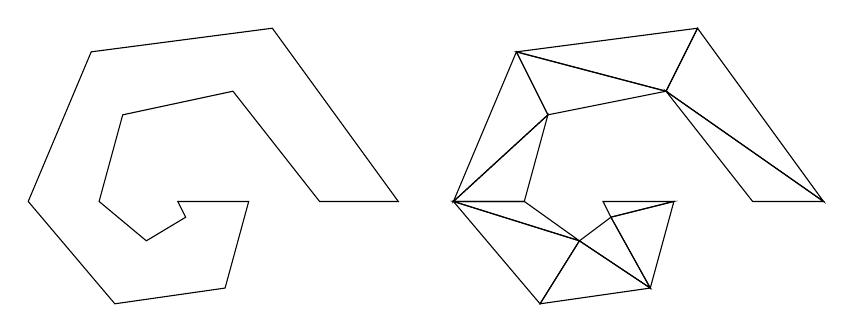
\begin{tikzpicture}
        \draw (1.3, 1.5) -- (1.6, 2.6) -- (3.0, 2.9) -- (4.1, 1.5) -- (5.1, 1.5) -- (3.5, 3.7) -- (1.2, 3.4) -- (0.4, 1.5) -- (1.5, 0.2) -- (2.9, 0.4) -- (3.2, 1.5) -- (2.3, 1.5) -- (2.4, 1.3) -- (1.9, 1.0) -- cycle;

        \pause
        \draw (7.8, 1.3) -- (7.4, 1.0) -- (8.3, 0.4) -- cycle;
        \draw (7.8, 1.3) -- (8.3, 0.4) -- (8.6, 1.5) -- cycle;
        \draw (7.8, 1.3) -- (8.6, 1.5) -- (7.7, 1.5) -- cycle;
        \draw (6.9, 0.2) -- (8.3, 0.4) -- (7.4, 1.0) -- cycle;
        \draw (6.9, 0.2) -- (7.4, 1.0) -- (5.8, 1.5) -- cycle;
        \draw (5.8, 1.5) -- (7.4, 1.0) -- (6.7, 1.5) -- cycle;
        \draw (5.8, 1.5) -- (6.7, 1.5) -- (7.0, 2.6) -- cycle;
        \draw (5.8, 1.5) -- (7.0, 2.6) -- (6.6, 3.4) -- cycle;
        \draw (7.0, 2.6) -- (8.5, 2.9) -- (6.6, 3.4) -- cycle;
        \draw (9.6, 1.5) -- (10.5, 1.5) -- (8.5, 2.9) -- cycle;
        \draw (8.9, 3.7) -- (6.6, 3.4) -- (8.5, 2.9) -- cycle;
        \draw (8.9, 3.7) -- (8.5, 2.9) -- (10.5, 1.5) -- cycle;
      \end{tikzpicture}
      \caption{Podział wielokąta na trójkąty}
    \end{figure}
  \end{center}
\end{frame}

\subsection{Problem galerii sztuki}
\begin{frame}
  \frametitle{Problem galerii sztuki}
  \begin{definition}
    Problem galerii sztuki to problem optymalizacyjny polegający na określeniu minimalnej liczby punktów obserwacyjnych (strażników) potrzebnych do monitorowania całego obszaru galerii sztuki.

    \pause
    Galerię sztuki modeluje się jako prosty wielokąt, a strażników jako punkty wewnątrz tego wielokąta. Zbiór $S$ punktów obserwacyjnych uważamy za pokrywający wielokąt $P$, jeśli dla każdego punktu wewnątrz $P$ istnieje punkt w $S$ taki, że odcinek łączący te dwa punkty nie przecina krawędzi wielokąta $P$.
  \end{definition}

  \pause
  \begin{figure}
    \includegraphics[scale=0.3]{art-gallery-problem}
    \caption{Czterech strażników monitorujących całą galerię sztuki}
  \end{figure}
\end{frame}

\begin{frame}
  \frametitle{Problem galerii sztuki}

  \begin{theorem}[Twierdzenie Chvátala]
    Aby cały prosty wielokąt z $n$ wierzchołkami był monitorowany, zawsze wystarczy co najwyżej $\lfloor n/3 \rfloor$ strażników. \qed
  \end{theorem}

  \only<2>{
    Powyższe twierdzenie wynika z faktu, że w procesie triangulacji każdy wielokąt prosty możemy podzielić na trójkąty. Strażnik umieszczony w wierzchołku trójkąta może monitorować cały ten trójkąt. Jeśli \textbf{pokolorujemy wierzchołki triangulacji na trzy kolory}, to każdy z kolorów będzie występował dokładnie raz w każdym trójkącie. Wybieramy zatem kolor występujący najrzadziej, uzyskując w ten sposób zbiór $\lfloor n/3 \rfloor$ punktów.
  }
  \only<3>{
    \begin{figure}
      \includegraphics[scale=0.1]{3-coloring}
      \caption{Trójkolorowanie wierzchołków triangulacji wielokąta - niebieskie punkty to strażnicy}
    \end{figure}
  }
\end{frame}

\subsection{Diagramy Voronoi}
\begin{frame}
  \frametitle{Diagramy Voronoi}
  \begin{definition}
    Teselacja to pokrycie płaszczyzny za pomocą wielokątów przylegających do siebie oraz nie nakładających się.
  \end{definition}

  \begin{definition}
    Diagram Voronoi to \textbf{podział płaszczyzny na obszary w oparciu o odległość do określonego zbioru punktów}. Każdy obszar składa się z punktów bliższych do jednego punktu z danego zbioru niż do jakiegokolwiek innego punktu ze zbioru. Jest to przykład tesselacji płaszczyzny.
  \end{definition}

  \pause
  Diagramy te zostały nazwane na cześć matematyka Gieorgija Woronoja, rosyjskiego matematyka ukraińskiego pochodzenia, który opisał je w 1908 roku.
\end{frame}

\begin{frame}
  \frametitle{Diagramy Voronoi}
  Niech $P = \{p_1, p_2, \ldots, p_n\}$, gdzie $p_i \in \mathbb{R}^2, n \in \mathbb{N}$.
  Punkty ze zbioru $P$ nazywać będziemy centrami.

  \begin{definition}
    Komórką diagramu Voronoi dla punktu $p_i$ nazywamy
    \begin{center}
      $V_P(p_i) = \{x : \forall_{j \neq i} d(x, p_i) \leq d(x, p_j) \}$
    \end{center}
    gdzie $d$ jest funkcją odległości między punktami.
  \end{definition}

  \pause
  \begin{definition}
    Podział płaszczyzny na $n$ komórek Voronoi $V_P(p_1), V_P(p_2), \ldots, V_P(p_n)$ nazywamy diagramem Voronoi dla zbioru punktów $P$. Oznaczamy go jako $Vor(P)$.
  \end{definition}
\end{frame}

\begin{frame}
  \frametitle{Diagramy Voronoi - przykład}
  \begin{center}
    \begin{figure}
      \includegraphics<1>[scale=0.4]{voronoi-animation-0}
      \includegraphics<2>[scale=0.4]{voronoi-animation-1}
      \includegraphics<3>[scale=0.4]{voronoi-animation-2}
      \caption{Przykład diagramu Voronoi dla metryki euklidesowej}
    \end{figure}
  \end{center}
\end{frame}

\subsection{Diagramy Voronoi - porównanie metryk}
\begin{frame}
  \frametitle{Diagramy Voronoi - porównanie metryk}

  Do najpopularniejszych metryk używanych w diagramach Voronoi należą:
  \begin{itemize}
    \item Metryka euklidesowa \\
      $d[(a_1, a_2), (b_1, b_2)] = \sqrt{(a_1 - b_1)^2 + (a_2 - b_2)^2}$
    \item Metryka Manhattan \\
      $d[(a_1, a_2), (b_1, b_2)] = |a_1 - b_1| + |a_2 - b_2|$
    \item Metryka Czebyszewa \\
      $d[(a_1, a_2), (b_1, b_2)] = \max(|a_1 - b_1|, |a_2 - b_2|)$
  \end{itemize}
\end{frame}

\begin{frame}
  \frametitle{Diagramy Voronoi - porównanie metryk}
  \begin{center}
    \begin{figure}
      \includegraphics<1>[scale=0.35]{voronoi_euklidesowa}
      \includegraphics<2>[scale=0.35]{voronoi_manhattan}
      \includegraphics<3>[scale=0.35]{voronoi_czebyszewa}
      \only<1>{\caption{Diagram Voronoi dla metryki euklidesowej}}
      \only<2>{\caption{Diagram Voronoi dla metryki Manhattan}}
      \only<3>{\caption{Diagram Voronoi dla metryki Czebyszewa}}
    \end{figure}
  \end{center}
\end{frame}

\begin{frame}
  \frametitle{Diagramy Voronoi - algorytmy tworzenia}
  Do najpopularniejszych sposobów tworzenia diagramów Voronoi należą:
  \begin{itemize}
    \item \color<1>{violet}{\textbf{Algorytm Fortune'a} - najczęściej stosowany, pozwala na zbudowanie diagramu Voronoi w czasie $O(n \log n)$ dla $n$ punktów wejściowych. Jest to algorytm zamiatający - linia omija zbiór punktów w określonym kierunku, a kiedy wszystkie punkty zostaną przetworzone, tworzony jest diagram Voronoi.}
      \pause
    \item \color<2>{violet}{\textbf{Obliczanie triangulacji Delaunaya} (\textit{Delone}) i tworzenie diagramu Voronoi na jej podstawie. Złożoność: $O(n \log n)$.}
  \end{itemize}
\end{frame}

\subsection{Algorytm Fortune'a}
\begin{frame}
  \frametitle{Algorytm Fortune'a}
  Algorytm Fortune'a to \textbf{algorytm zamiatający} (\textit{sweep line algorithm}), pozwalający na efektywne tworzenie diagramów Voronoi w czasie $O(n \log n)$ wykorzystując $O(n)$ pamięci dla $n$ punktów wejściowych.
\end{frame}

\begin{frame}
  \frametitle{Algorytm Fortune'a - zasada działania}

  \begin{definition}
    Parabola to krzywa będąca zbiorem punktów równoodległych od prostej zwanej kierownicą paraboli i punktu zwanego ogniskiem paraboli.
  \end{definition}

  \pause
  \begin{figure}
    \includegraphics[scale=0.1]{parabola}
    \caption{Wizualizacja paraboli jako zbioru punktów równoodległych od prostej $l$ oraz punktu $F$}
  \end{figure}
\end{frame}

\begin{frame}
  \frametitle{Algorytm Fortune'a - definicje}
  \begin{definitions}
    \textbf{Linia zamiatająca} (\textit{sweep line}) - linia prosta, przesuwająca się wzdłuż płaszczyzny, przetwarzająca punkty wejściowe.

    \textbf{Linia plażowa} (\textit{beach line}) - krzywa utworzona przez punkty równoodległe od linii zamiatającej i najbliższe z punktów już przetworzonych. Składa się z łuków parabolicznych.

    \textbf{Zdarzenia punktowe} (\textit{point events}) - miejsca, w których linia zamiatająca napotyka punkty wejściowe.

    \textbf{Zdarzenia wierzchołkowe} (\textit{vertex events}) - miejsca, w których zanikają łuki paraboliczne na linii plażowej.
  \end{definitions}

  \begin{center}
    \begin{figure}
      \includegraphics[scale=0.4]{sweep-beach-line}
      \caption{Linia zamiatająca i linia plażowa}
    \end{figure}
  \end{center}
\end{frame}

\begin{frame}
  \frametitle{Algorytm Fortune'a - zasada działania}
  \begin{itemize}
    \item Punkty znajdujące się \textbf{za linią zamiatającą nie mają wpływu na kształt linii plażowej}, gdyż nigdy nie będą spełniać warunku bycia najbliższym punktem dla żadnego punktu przed linią zamiatającą.
      \pause
    \item W trakcie działania algorytmu przesuwana jest linia zamiatająca wzdłuż płaszczyzny. Gdy \textbf{linia napotyka nowy punkt, tworzony jest nowy łuk paraboliczny} na linii plażowej, ponieważ ten punkt staje się najbliższym punktem dla pewnego obszaru przed linią zamiatającą. Zdarzenie to nazywane jest zdarzeniem punktowym.
  \end{itemize}

  \begin{center}
    \begin{figure}
      \includegraphics[scale=0.5]{point-event}
      \caption{Zdarzenie punktowe - dodanie nowego łuku parabolicznego}
    \end{figure}
  \end{center}
\end{frame}

\begin{frame}
  \frametitle{Algorytm Fortune'a - zasada działania}
  \begin{itemize}
    \item W trakcie przesuwania linii zamiatającej, łuki paraboliczne tworzące linię plażową będą się zmieniać. Gdy \textbf{linia zamiatająca osiągnie punkt, w którym trzy łuki paraboliczne stykają się w jednym punkcie, środkowy łuk zniknie}, a dwa pozostałe połączą się. Zdarzenie to nazywane jest zdarzeniem wierzchołkowym.
      \pause
    \item Efektem zdarzenia wierzchołkowego jest \textbf{utworzenie nowego wierzchołka diagramu Voronoi}, ponieważ punkt styku trzech łuków parabolicznych jest równoodległy od trzech punktów wejściowych.
  \end{itemize}

  \begin{center}
    \begin{figure}
      \includegraphics[scale=0.7]{vertex-event}
      \caption{Zdarzenie wierzchołkowe}
    \end{figure}
  \end{center}
\end{frame}

\begin{frame}
  \frametitle{Algorytm Fortune'a - animacja}
  \begin{center}
    \begin{figure}
      \includegraphics<1>[scale=0.4]{fortunes-animation-0}
      \includegraphics<2>[scale=0.4]{fortunes-animation-1}
      \includegraphics<3>[scale=0.4]{fortunes-animation-2}
      \includegraphics<4>[scale=0.4]{fortunes-animation-3}
      \includegraphics<5>[scale=0.4]{fortunes-animation-4}
      \includegraphics<6>[scale=0.4]{fortunes-animation-5}
      \includegraphics<7>[scale=0.4]{fortunes-animation-6}
      \includegraphics<8>[scale=0.4]{fortunes-animation-7}
      \caption{Przykład działania algorytmu Fortune'a - animacja dostępna pod adresem: \url{https://jacquesheunis.com/post/fortunes-algorithm/}}
    \end{figure}
  \end{center}
\end{frame}

\begin{frame}
  \frametitle{Algorytm Fortune'a - ilość paraboli na linii plażowej}
  Jak można zauważyć na przedstawionym przykładzie, każde zdarzenie punktowe powoduje dodanie nowego łuku parabolicznego na linii plażowej, jednocześnie mogąc powodować podział istniejącego łuku na dwa mniejsze łuki. W takim przypadku \textbf{zdarzenie punktowe może powodować zwiększenie liczby łuków na linii plażowej o maksymalnie dwa.}
  Warto zauważyć, że dla pierwszego punktu zawsze tworzony jest dokładnie jeden łuk paraboliczny.

  \pause
  \begin{theorem}
    Dla zbioru $n$ punktów wejściowych, linia plażowa w algorytmie Fortune'a może składać się z maksymalnie $2n - 1$ łuków parabolicznych. \qed
  \end{theorem}
\end{frame}

\begin{frame}
  \frametitle{Algorytm Fortune'a - struktury danych}
  Algorytm Fortune'a wykorzystuje dwie główne struktury danych:
  \begin{itemize}
    \item \textbf{Kolejka priorytetowa} - przechowuje zdarzenia punktowe i wierzchołkowe, posortowane według ich pozycji na osi wzdłuż której przesuwa się linia zamiatająca.
      \pause
    \item \textbf{Drzewo binarne} - reprezentuje linię plażową, przechowując łuki paraboliczne w kolejności od lewej do prawej jako węzły drzewa.
  \end{itemize}

  \begin{center}
    \begin{figure}
      \includegraphics[scale=0.4]{beach-line-binary-tree}
      \caption{Proces dodawania reprezentacji nowej paraboli do drzewa binarnego opisującego linię plażową}
    \end{figure}
  \end{center}
\end{frame}

\subsection{Algorytm Fortune'a - pseudokod}
\begin{frame}
  \frametitle{Algorytm Fortune'a - pseudokod}

  \begin{algorithm}[H]
    \caption{Algorytm Fortune'a}
    \begin{algorithmic}
      \Function{voronoiFortune}{punkty}
      \State $kolejkaZdarzen \gets$ zdarzenia punktowe utworzone z $punkty$
      \State $liniaPlazowa \gets$ puste drzewo binarne
      \State $diagramVoronoi \gets$ pusty diagram Voronoi

      \While {kolejkaZdarzen nie jest pusta}
      \State $zdarzenie \gets$ usuń pierwsze zdarzenie z $kolejkaZdarzen$
      \If{$zdarzenie$ jest zdarzeniem punktowym}
      \State dodajParabolę($zdarzenie$)
      \Else
      \State usuńParabolę($zdarzenie$)
      \EndIf
      \EndWhile
      \EndFunction
    \end{algorithmic}
  \end{algorithm}
\end{frame}

\begin{frame}
  \frametitle{Algorytm Fortune'a - pseudokod}

  \begin{algorithm}[H]
    \caption{Algorytm Fortune'a - dodajParabolę}
    \begin{algorithmic}
      \Function{dodajParabolę}{$zdarzenie$}
      \If{$liniaPlazowa$ jest pusta} dodaj nową parabolę do $liniaPlazowa$ i zakończ funkcję \EndIf
      \State
      \State $parabola$ $\gets$ parabola znajdująca się pod punktem $zdarzenie$
      \State \textbf{usuń} z $kolejkaZdarzen$ wszelkie zdarzenia wierzchołkowe związane z $parabola$
      \State
      \State \textbf{podziel} $parabola$ na dwa mniejsze łuki i dodaj nową parabolę między nimi do $liniaPlazowa$
      \State sprawdź czy dla nowych łuków \textbf{istnieją zdarzenia wierzchołkowe} (czyli jeden z łuków zanika, bo odległość od 3 punktów jest równa) i dodaj je do $kolejkaZdarzen$
      \EndFunction
    \end{algorithmic}
  \end{algorithm}
\end{frame}

\begin{frame}
  \frametitle{Algorytm Fortune'a - pseudokod}

  \begin{algorithm}[H]
    \caption{Algorytm Fortune'a - usuńParabolę}
    \begin{algorithmic}
      \Function{usuńParabolę}{$zdarzenie$}
      \State $lewaParabola, prawaParabola \gets$ parabolę po lewej i prawej stronie paraboli znikającej w zdarzeniu $zdarzenie$
      \State \textbf{usuń} z $kolejkaZdarzen$ wszelkie zdarzenia wierzchołkowe związane z $lewaParabola$ i $prawaParabola$
      \State
      \State $srodekOkregu \gets$ punkt styku łuków parabolicznych w zdarzeniu $zdarzenie$
      \State \textbf{dodaj} nowy wierzchołek do $diagramVoronoi$ w $srodekOkregu$
      \State
      \State \textbf{usuń} parabolę znikającą w zdarzeniu $zdarzenie$ z $liniaPlazowa$
      \State sprawdź czy dla $lewaParabola$ i $prawaParabola$ \textbf{istnieje zdarzenie wierzchołkowe} i dodaj je do $kolejkaZdarzen$
      \EndFunction
    \end{algorithmic}
  \end{algorithm}
\end{frame}

\subsection{Algorytm Fortune'a - oszacowanie złożoności i dowód}
\begin{frame}
  \frametitle{Algorytm Fortune'a - oszacowanie złożoności i dowód}

  \begin{theorem}
    Każdy wierzchołek diagramu Voronoi jest co najmniej stopnia trzeciego. \qed
  \end{theorem}

  \begin{theorem}
    Algorytm Fortune'a tworzy diagram Voronoi dla $n$ punktów wejściowych w czasie $O(n \log n)$ wykorzystując $O(n)$ pamięci.
  \end{theorem}
\end{frame}

\begin{frame}
  \frametitle{Algorytm Fortune'a - oszacowanie złożoności i dowód}
  \begin{small}
    \begin{proof}
      Niech $V$ będzie liczbą wierzchołków, $E$ liczbą krawędzi, a $N$ liczbą ścian diagramu Voronoi.

      Ponieważ diagram Voronoi posiada nieskończone ściany, \textbf{dodajemy do niego sztuczny wierzchołek} i łączymy go z wszystkimi nieskończonymi krawędziami, tworząc nowy graf planarny. Z \textbf{wzoru Eulera dla grafów planarnych} mamy $V - E + N = 2$. W takim razie $(V + 1) - E + N = 2$.
      \pause

      Każdy \textbf{wierzchołek diagramu Voronoi ma stopień co najmniej 3}, więc $3(V + 1) \leq 2E$. Po prostych przekształceniach otrzymujemy $V \leq 2N - 5$ oraz $E \leq 3N - 6$.

      \pause
      Liczba zdarzeń punktowych wynosi dokładnie $N$, a liczba zdarzeń wierzchołkowych $V$, którą możemy górnie ograniczyć przez $2N - 5$. Zatem \textbf{łączna liczba zdarzeń możemy oszacować przez $O(n)$}.

      Każde zdarzenie wywołuje stałą liczbę operacji $c$ na drzewie binarnym i kolejce priorytetowej. \textbf{Operacje te mają złożoność $O(\log n)$}. Zatem całkowity czas działania algorytmu wynosi $O(n \log n)$.
    \end{proof}
  \end{small}
\end{frame}

\subsection{Triangulacja Delaunaya}
\begin{frame}
  \frametitle{Triangulacja Delaunaya}

  \begin{definitions}
    \textbf{Otoczka wypukła} zbioru punktów to najmniejszy wypukły wielokąt, który zawiera wszystkie punkty ze zbioru.

    \textbf{Triangulacja Delaunaya} (\textit{Delone}) zbioru punktów dzieli ich otoczkę wypukłą na trójkąty w taki sposób, że \textbf{żaden punkt ze zbioru nie znajduje się wewnątrz okręgu opisanego na żadnym z trójkątów triangulacji}.
  \end{definitions}

  Nazwa Triangulacji Delaunaya pochodzi od rosyjskiego matematyka Borysa Delaunaya, który opisał ją w 1934 roku.
\end{frame}

\begin{frame}
  \frametitle{Triangulacja Delaunaya}
  W triangulacji Delaunaya dla zbioru punktów $P$:
  \begin{itemize}
    \item Każdy trójkąt ma swoje wierzchołki w punktach ze zbioru $P$.
    \item Dla każdego trójkąta, okrąg opisany na nim nie zawiera żadnego innego punktu ze zbioru $P$ wewnątrz siebie.
    \item Podział taki maksymalizuje minimalny kąt wszystkich trójkątów w triangulacji.
  \end{itemize}
\end{frame}

\begin{frame}
  \frametitle{Triangulacja Delaunaya - przykład}
  \begin{center}
    \begin{figure}
      \includegraphics[scale=0.19]{delaunay-0}
      \caption{Przykład triangulacji Delaunaya dla zbioru punktów}
    \end{figure}
  \end{center}
\end{frame}

\begin{frame}
  \frametitle{Triangulacja Delaunaya - algorytm Bowyera-Watsona}
  Jednym z algorytmów tworzenia triangulacji Delaunaya jest \textbf{algorytm Bowyera-Watsona}. Jest to algorytm przyrostowy, który działa poprzez dodawanie punktów jeden po drugim do triangulacji Delaunaya.
  \pause

  Po wstawieniu każdego punktu, wszystkie trójkąty, których okręgi opisane zawierają nowy punkt, są usuwane. Powstała luka jest następnie ponownie triangulowana z nowym punktem jako jednym z wierzchołków.

  \pause
  Algorytm ten ma średnią złożoność czasową równą $O(n \log n)$ oraz $O(n^2)$ w pesymistycznym przypadku dla $n$ punktów wejściowych.
\end{frame}

\begin{frame}
  \frametitle{Triangulacja Delaunaya - związek z diagramem Voronoi}

  Środek okręgu opisanego na trójkącie jest równoodległy od wszystkich trzech wierzchołków trójkąta. W takim razie jest to punkt, w którym trzy komórki Voronoi stykają się ze sobą. Wynika z tego bardzo ważna własność triangulacji Delaunaya i diagramu Voronoi:
  \pause
  \begin{theorem}
    Jeśli dwa trójkąty w triangulacji Delaunaya mają wspólną krawędź, to środki okręgów opisanych na tych trójkątach łączy się krawędzią w diagramie Voronoi. \qed
  \end{theorem}
\end{frame}

\begin{frame}
  \frametitle{Triangulacja Delaunaya - związek z diagramem Voronoi}
  \begin{center}
    \begin{figure}
      \includegraphics<1>[scale=0.19]{delaunay-1}
      \includegraphics<2>[scale=0.19]{delaunay-2}
      \only<1>{\caption{Triangulacja Delaunaya z zaznaczonymi na czerwono środkami okręgów opisanych na trójkątach}}
      \only<2>{\caption{Po połączeniu środków okręgów opisanych na stykających się trójkątach powstaje diagram Voronoi - zaznaczony na czerwono}}
    \end{figure}
  \end{center}
\end{frame}

\subsection{Zastosowania}
\begin{frame}
  \frametitle{Zastosowania}
  Triangulacja i diagramy Voronoi znajdują zastosowanie między innymi w:
  \begin{itemize}
    \item Planowaniu chirurgicznym i tworzeniu modeli 3D narządów
    \item Epidemiologii przestrzennej i analizie ognisk chorób
    \item Przedstawianiu struktury kosmicznej we wszechświecie
  \end{itemize}
\end{frame}

\begin{frame}
  \frametitle{Zastosowania}
  \begin{center}
    \only<1>{
      \begin{figure}
        \includegraphics[scale=0.3]{bone-triangulation}
        \caption{Triangulacja wykorzystana do przybliżenia kształtu kości ludzkiej w celu planowania chirurgicznego}
      \end{figure}
    }
    \only<2>{
      \begin{figure}
        \includegraphics[scale=0.4]{cholera-voronoi}
        \caption{Diagram Voronoi wykorzystany do analizy przestrzennej ogniska cholery w Londynie w 1854 roku}
      \end{figure}
    }
    \only<3>{
      \begin{figure}
        \includegraphics[scale=0.4]{3d-tesselation-cosmic-structure}
        \caption{Trójwymiarowa tesselacja wykorzystana do przedstawienia struktury kosmicznej we wszechświecie}
      \end{figure}
    }
  \end{center}
\end{frame}

\subsection{Źródła}
\begin{frame}
  \frametitle{Źródła}

  \only<1>{
    \begin{thebibliography}{9}
      \bibitem{1} \url{https://mathworld.wolfram.com/Triangulation.html}
      \bibitem{2} \url{https://en.wikipedia.org/wiki/Triangulation_(disambiguation)}
      \bibitem{3} \url{https://en.wikipedia.org/wiki/Planar_graph}
      \bibitem{4} \url{https://en.wikipedia.org/wiki/Chordal_graph}
      \bibitem{5} \url{https://en.wikipedia.org/wiki/Simplex}
      \bibitem{6} \url{https://facultyweb.kennesaw.edu/mlavrov/courses/graph-theory/lecture21.pdf}
      \bibitem{7} \url{https://mathworld.wolfram.com/Goldner-HararyGraph.html}
      \bibitem{8} \url{https://en.wikipedia.org/wiki/Voronoi_diagram}
      \bibitem{9} \url{https://en.wikipedia.org/wiki/Tessellation}
    \end{thebibliography}
  }
  \only<2>{
    \begin{thebibliography}{8}
      \bibitem{1} \url{https://www.math.us.edu.pl/lsim2014/MSerwecinska-lsim2014.pdf}
      \bibitem{2} \url{https://jacquesheunis.com/post/fortunes-algorithm/}
      \bibitem{3} \url{https://cs.sfu.ca/~binay/813.2011/Fortune.pdf}
      \bibitem{4} \url{https://blog.ivank.net/fortunes-algorithm-and-implementation.html}
      \bibitem{5} \url{https://en.wikipedia.org/wiki/Delaunay_triangulation}
      \bibitem{6} \url{https://ianthehenry.com/posts/delaunay/}
      \bibitem{7} \url{https://plus.maths.org/content/uncovering-cause-cholera}
      \bibitem{8} \url{https://www.researchgate.net/publication/221909127_Finite_Element_Analysis_in_Orthopaedic_Biomechanics}
    \end{thebibliography}
  }
  \only<3>{
    \begin{thebibliography}{3}
      \bibitem{1} \url{https://www.astro.rug.nl/~weygaert/tim1publication/vorwey.isvd07.pdf}
      \bibitem{2} \url{https://en.wikipedia.org/wiki/Bowyer-Watson_algorithm}
      \bibitem{3} \url{https://en.wikipedia.org/wiki/Art_gallery_problem}
    \end{thebibliography}
  }
\end{frame}

\end{document}
